% Options for packages loaded elsewhere
\PassOptionsToPackage{unicode}{hyperref}
\PassOptionsToPackage{hyphens}{url}
%
\documentclass[
]{book}
\title{Estadística Aplicada a las Ciencias y la Ingeniería}
\author{Emilio L. Cano}
\date{2021-09-23}

\usepackage{amsmath,amssymb}
\usepackage{lmodern}
\usepackage{iftex}
\ifPDFTeX
  \usepackage[T1]{fontenc}
  \usepackage[utf8]{inputenc}
  \usepackage{textcomp} % provide euro and other symbols
\else % if luatex or xetex
  \usepackage{unicode-math}
  \defaultfontfeatures{Scale=MatchLowercase}
  \defaultfontfeatures[\rmfamily]{Ligatures=TeX,Scale=1}
\fi
% Use upquote if available, for straight quotes in verbatim environments
\IfFileExists{upquote.sty}{\usepackage{upquote}}{}
\IfFileExists{microtype.sty}{% use microtype if available
  \usepackage[]{microtype}
  \UseMicrotypeSet[protrusion]{basicmath} % disable protrusion for tt fonts
}{}
\makeatletter
\@ifundefined{KOMAClassName}{% if non-KOMA class
  \IfFileExists{parskip.sty}{%
    \usepackage{parskip}
  }{% else
    \setlength{\parindent}{0pt}
    \setlength{\parskip}{6pt plus 2pt minus 1pt}}
}{% if KOMA class
  \KOMAoptions{parskip=half}}
\makeatother
\usepackage{xcolor}
\IfFileExists{xurl.sty}{\usepackage{xurl}}{} % add URL line breaks if available
\IfFileExists{bookmark.sty}{\usepackage{bookmark}}{\usepackage{hyperref}}
\hypersetup{
  pdftitle={Estadística Aplicada a las Ciencias y la Ingeniería},
  pdfauthor={Emilio L. Cano},
  hidelinks,
  pdfcreator={LaTeX via pandoc}}
\urlstyle{same} % disable monospaced font for URLs
\usepackage{color}
\usepackage{fancyvrb}
\newcommand{\VerbBar}{|}
\newcommand{\VERB}{\Verb[commandchars=\\\{\}]}
\DefineVerbatimEnvironment{Highlighting}{Verbatim}{commandchars=\\\{\}}
% Add ',fontsize=\small' for more characters per line
\usepackage{framed}
\definecolor{shadecolor}{RGB}{248,248,248}
\newenvironment{Shaded}{\begin{snugshade}}{\end{snugshade}}
\newcommand{\AlertTok}[1]{\textcolor[rgb]{0.94,0.16,0.16}{#1}}
\newcommand{\AnnotationTok}[1]{\textcolor[rgb]{0.56,0.35,0.01}{\textbf{\textit{#1}}}}
\newcommand{\AttributeTok}[1]{\textcolor[rgb]{0.77,0.63,0.00}{#1}}
\newcommand{\BaseNTok}[1]{\textcolor[rgb]{0.00,0.00,0.81}{#1}}
\newcommand{\BuiltInTok}[1]{#1}
\newcommand{\CharTok}[1]{\textcolor[rgb]{0.31,0.60,0.02}{#1}}
\newcommand{\CommentTok}[1]{\textcolor[rgb]{0.56,0.35,0.01}{\textit{#1}}}
\newcommand{\CommentVarTok}[1]{\textcolor[rgb]{0.56,0.35,0.01}{\textbf{\textit{#1}}}}
\newcommand{\ConstantTok}[1]{\textcolor[rgb]{0.00,0.00,0.00}{#1}}
\newcommand{\ControlFlowTok}[1]{\textcolor[rgb]{0.13,0.29,0.53}{\textbf{#1}}}
\newcommand{\DataTypeTok}[1]{\textcolor[rgb]{0.13,0.29,0.53}{#1}}
\newcommand{\DecValTok}[1]{\textcolor[rgb]{0.00,0.00,0.81}{#1}}
\newcommand{\DocumentationTok}[1]{\textcolor[rgb]{0.56,0.35,0.01}{\textbf{\textit{#1}}}}
\newcommand{\ErrorTok}[1]{\textcolor[rgb]{0.64,0.00,0.00}{\textbf{#1}}}
\newcommand{\ExtensionTok}[1]{#1}
\newcommand{\FloatTok}[1]{\textcolor[rgb]{0.00,0.00,0.81}{#1}}
\newcommand{\FunctionTok}[1]{\textcolor[rgb]{0.00,0.00,0.00}{#1}}
\newcommand{\ImportTok}[1]{#1}
\newcommand{\InformationTok}[1]{\textcolor[rgb]{0.56,0.35,0.01}{\textbf{\textit{#1}}}}
\newcommand{\KeywordTok}[1]{\textcolor[rgb]{0.13,0.29,0.53}{\textbf{#1}}}
\newcommand{\NormalTok}[1]{#1}
\newcommand{\OperatorTok}[1]{\textcolor[rgb]{0.81,0.36,0.00}{\textbf{#1}}}
\newcommand{\OtherTok}[1]{\textcolor[rgb]{0.56,0.35,0.01}{#1}}
\newcommand{\PreprocessorTok}[1]{\textcolor[rgb]{0.56,0.35,0.01}{\textit{#1}}}
\newcommand{\RegionMarkerTok}[1]{#1}
\newcommand{\SpecialCharTok}[1]{\textcolor[rgb]{0.00,0.00,0.00}{#1}}
\newcommand{\SpecialStringTok}[1]{\textcolor[rgb]{0.31,0.60,0.02}{#1}}
\newcommand{\StringTok}[1]{\textcolor[rgb]{0.31,0.60,0.02}{#1}}
\newcommand{\VariableTok}[1]{\textcolor[rgb]{0.00,0.00,0.00}{#1}}
\newcommand{\VerbatimStringTok}[1]{\textcolor[rgb]{0.31,0.60,0.02}{#1}}
\newcommand{\WarningTok}[1]{\textcolor[rgb]{0.56,0.35,0.01}{\textbf{\textit{#1}}}}
\usepackage{longtable,booktabs,array}
\usepackage{calc} % for calculating minipage widths
% Correct order of tables after \paragraph or \subparagraph
\usepackage{etoolbox}
\makeatletter
\patchcmd\longtable{\par}{\if@noskipsec\mbox{}\fi\par}{}{}
\makeatother
% Allow footnotes in longtable head/foot
\IfFileExists{footnotehyper.sty}{\usepackage{footnotehyper}}{\usepackage{footnote}}
\makesavenoteenv{longtable}
\usepackage{graphicx}
\makeatletter
\def\maxwidth{\ifdim\Gin@nat@width>\linewidth\linewidth\else\Gin@nat@width\fi}
\def\maxheight{\ifdim\Gin@nat@height>\textheight\textheight\else\Gin@nat@height\fi}
\makeatother
% Scale images if necessary, so that they will not overflow the page
% margins by default, and it is still possible to overwrite the defaults
% using explicit options in \includegraphics[width, height, ...]{}
\setkeys{Gin}{width=\maxwidth,height=\maxheight,keepaspectratio}
% Set default figure placement to htbp
\makeatletter
\def\fps@figure{htbp}
\makeatother
\setlength{\emergencystretch}{3em} % prevent overfull lines
\providecommand{\tightlist}{%
  \setlength{\itemsep}{0pt}\setlength{\parskip}{0pt}}
\setcounter{secnumdepth}{5}
\usepackage{booktabs}
\usepackage[spanish, es-tabla]{babel}

\usepackage{tcolorbox}

\usepackage{tikz}
\definecolor{ejemplob}{RGB}{238,238,238}
\definecolor{ejemplof}{RGB}{204,204,204}
\definecolor{practicab}{RGB}{255,243,205}
\definecolor{practicaf}{RGB}{255,238,186}
\definecolor{premiumb}{RGB}{248,215,218}
\definecolor{premiumf}{RGB}{245,198,203}

\newtcolorbox{rmdejemplo}{
  colback=ejemplob,
  colframe=ejemplof,
  coltext=black,
  boxsep=5pt,
  left = 25pt,
  arc=4pt,
  % overlay={\node[inner sep=0pt, xshift=.85cm, anchor=center] 
  %   at ($ (frame.north west)!.5!(frame.south west) $) {
\includegraphics[width=6mm]{images/ejemplo}}; }}
  overlay={{
\includegraphics[width=8mm]{images/ejemplo}}; }}

\newtcolorbox{rmdcafe}{
  colback=ejemplob,
  colframe=ejemplof,
  coltext=black,
  boxsep=5pt,
  left = 25pt,
  arc=4pt,
  % overlay={\node[inner sep=0pt, xshift=.85cm, anchor=center] 
  %   at ($ (frame.north west)!.5!(frame.south west) $) {
\includegraphics[width=6mm]{images/ejemplo}}; }}
  overlay={{
\includegraphics[width=8mm]{images/cafe}}; }}

\newtcolorbox{rmdpractica}{
  colback=practicab,
  colframe=practicaf,
  coltext=black,
  boxsep=5pt,
  left = 25pt,
  arc=4pt,
  % overlay={\node[inner sep=0pt, xshift=.85cm, anchor=center] 
  %   at ($ (frame.north west)!.5!(frame.south west) $) {
\includegraphics[width=6mm]{images/ejemplo}}; }}
  overlay={{
\includegraphics[width=8mm]{images/practice}}; }}

\newtcolorbox{rmdpremium}{
  colback=ejemplob,
  colframe=ejemplof,
  coltext=black,
  boxsep=5pt,
  left = 25pt,
  arc=4pt,
  % overlay={\node[inner sep=0pt, xshift=.85cm, anchor=center] 
  %   at ($ (frame.north west)!.5!(frame.south west) $) {
\includegraphics[width=6mm]{images/ejemplo}}; }}
  overlay={{
\includegraphics[width=8mm]{images/premium}}; }}


\ifLuaTeX
  \usepackage{selnolig}  % disable illegal ligatures
\fi
\usepackage[]{natbib}
\bibliographystyle{apalike}

\begin{document}
\maketitle

{
\setcounter{tocdepth}{1}
\tableofcontents
}
\hypertarget{bienvenida}{%
\chapter*{Bienvenida}\label{bienvenida}}
\addcontentsline{toc}{chapter}{Bienvenida}

Este libro incluye los contenidos habitualmente presentes en el currículo
de asignaturas de \textbf{Estadística} de los grados Ciencias e Ingenierías de universidades españolas. Aunque no aparezca en el título, el manual incluye también los contenidos de \textbf{Probabilidad} necesarios.
Si bien existe abundante material bibliográfico
que cubre los contenidos de estas asignaturas, quería elaborar un material
propio que no fuera solamente para mis clases sino algo más
\emph{global}. En los últimos años ya lo hice para asignaturas de grado y Máster en ADE \citep{libroeee, libroadr}. Por otra parte, me motiva cubrir el hueco de los materiales
de acceso gratuito con la opción de comprar una edición
impresa\footnote{A la espera de encontrar editorial.} y con el enfoque
que se menciona en el siguiente apartado. Por otra parte, los libros publicados
originalmente en inglés y traducidos al español a menudo me resultan lejanos
a nuestro idioma (por muy buenas que sean las traducciones, los ejemplos en \emph{acres}
no son muy intuitivos para un lector español). Espero que también sirva para
lectores de otros países de habla hispana.

\hypertarget{estuxe1ndares-y-software}{%
\section*{Estándares y software}\label{estuxe1ndares-y-software}}
\addcontentsline{toc}{section}{Estándares y software}

Los contenidos de este libro se basan en dos paradigmas que están presentes
en los intereses de investigación y docencia del autor: los \textbf{estándares} y
el \textbf{software libre}. En lo que se refiere a estándares, la notación utilizada,
definiciones y fórmulas se ajustarán el máximo posible a la utilizada en normas
nacionales e internacionales sobre metodología estadística. Estas normas se
citarán pertinentemente a lo largo del texto. En cuanto al software libre,
se proporcionarán instrucciones para resolver los ejemplos
que ilustran la teoría utilizando software libre.
No obstante, el uso del software es
auxiliar al texto y se puede seguir sin necesidad de utilizar
los programas. Según lo que proceda en cada caso, se utilizará
software de hoja de cálculo, el software estadístico y lenguaje de
programación
\textbf{R} \citep{R-base},
y el software de álgebra computacional \textbf{Máxima}\footnote{\url{http://maxima.sourceforge.net/es/}}.
Respecto al software de hoja de cálculo, las fórmulas utilizadas se han probado
en el software libre \textbf{LibreOffice}\footnote{\url{https://es.libreoffice.org}}, en \textbf{Hojas de Cálculo de Google}\footnote{\url{https://www.google.es/intl/es/sheets/about/}} y
también en \textbf{Microsoft EXCEL}\footnote{\url{https://products.office.com/es-es/excel}} que,
aunque no es software libre, su uso
está más que generalizado y normalmente los estudiantes disponen de licencia de uso
a través de su universidad. En caso de que el nombre de la función sea distinta
en EXCEL, se indicará en el propio ejemplo.

Las normas son clave para el desarrollo económico de un país. Estudios en diversos países,
incluido España, han demostrado que la aportación de la normalización a su economía es del 1\% del PIB\footnote{\url{http://www.aenor.es/DescargasWeb/normas/como-beneficia-es.pdf}}. La
Asociación Española de Normalización (UNE) es el organismo legalmente
responsable del desarrollo y difusión de las normas técnicas en España.
Además, representa a España en los organismos internacionales de normalización como
\href{https://www.iso.org/}{ISO}\footnote{\url{https://www.iso.org/}} y \href{https://www.cen.eu/}{CEN}\footnote{\url{https://www.cen.eu/}}.

Las normas sobre estadística que surgen de ISO las elabora el \emph{Technical Committee}
ISO TC 69\footnote{\url{https://www.iso.org/committee/49742/x/catalogue/}} \emph{Statistical Methods}.
Por su parte, el subcomité técnico de normalización
CTN 66/SC 3\footnote{\url{https://www.une.org/encuentra-tu-norma/comites-tecnicos-de-normalizacion/comite/?c=CTN\%2066/SC\%203}}, Métodos Estadísticos,
participa como miembro nacional en ese comité ISO.
Las normas que son de interés en España, se ratifican en inglés o se traducen
al español como normas UNE. Para una descripción más completa de la elaboración
de normas, véase \citet{cano2015qcr}.

\hypertarget{estructura-del-libro}{%
\section*{Estructura del libro}\label{estructura-del-libro}}
\addcontentsline{toc}{section}{Estructura del libro}

Este libro se ha elaborado utilizando el lenguaje \emph{Markdown} con el propio
software \textbf{R} y el paquete \textbf{bookdown} \citep{R-bookdown}.
Se incluyen una gran cantidad de ejemplos resueltos tanto de forma analítica
como mediante software. En algunos casos se proporciona el uso de funciones
en hojas de cálculo (y el resultado obtenido con un recuadro).
En otros, código de R, que aparecen en el texto
sombreados y con la sintaxis coloreada, como el fragmento a continuación
donde se puede comprobar la sesión de R en la que ha sido generado este material.
Obsérvese que los resultados se muestran precedidos de los símbolos
\texttt{\#\textgreater{}}.\texttt{\{r\}\ sessionInfo()}

Normalmente, la descripción o enunciado de los ejemplos se incluyen en bloques
con el siguiente aspecto:

\begin{rmdejemplo}
Esto es un ejemplo. A continuación puede mostrarse código o no. Los ejemplos
pueden ir precedidos por un icono para identificar su campo de aplicación, por
ejemplo \includegraphics[width=1em,height=1em]{index_files/figure-latex/fa-icon-37b8d5b2b6c465edf79712060e1bfd05.pdf} Biología, \includegraphics[width=1em,height=1em]{index_files/figure-latex/fa-icon-16880cffb899f7035dd670b3367c6a26.pdf} Ciencia y tecnología de Alimentos, o \includegraphics[width=0.75em,height=1em]{index_files/figure-latex/fa-icon-cad1ca165b8df24cf4a6670c9354ee87.pdf} Ciencia e Ingeniería Ambiental.

\end{rmdejemplo}

Cuando el ejemplo incluya explicaciones sobre cómo resolverlo con software,
estas explicaciones aparecerán en bloques con el siguiente aspecto:

\begin{rmdpractica}
\textbf{HOJA DE CÁLCULO}

La función \texttt{FACT} obtiene el factorial de un número x (\(x!\)):

\texttt{=FACT(5)}
\(\boxed{\mathsf{120}}\)

\end{rmdpractica}

También se incluirán con el formato anterior indicaciones para usar la calculadora
científica, cuando esto sea posible.

El texto incluye otros bloques con información de distinto tipo, como los siguientes:

\begin{rmdpremium}
Este contenido se considera avanzado. El lector principiante puede saltarse estos apartados
y volver sobre ellos en una segunda lectura.

\end{rmdpremium}

\begin{rmdcafe}
Estos bloques están pensados para incluir información curiosa o complementaria
para poner en contexto las explicaciones.

\end{rmdcafe}

Este volumen cubre los contenidos de asignaturas básicas de Estadística en un
amplio rango de grados. Puede servir también como repaso
para alumnos de posgrado o incluso egresados que necesiten refrescar
conocimientos o aprender a aplicarlos con software moderno. Un segundo volumen cubrirá en el futuro métodos y modelos avanzados para
entornos más exigentes.

El libro está dividido en 4 partes. La primera parte está dedicada a la Estadística
Descriptiva, y consta de un \protect\hyperlink{intro}{capítulo introductorio} seguido de sendos capítulos
para el análisis exploratorio univariante y bivariante. La segunda parte
trata la Probabilidad en 4 capítulos, uno introductorio, dos dedicados a las
variables
aleatorias univariantes y bivariantes respectivamente, y finalmente un capítulo
que trata los modelos de distribución de probabilidad. En la tercera parte se
aborda la inferencia estadística, con una introducción al muestreo y la
estimación puntual, seguida de capítulos dedicados a los contrastes de
comparación de grupos, análisis de regresión y diseño de experimentos. La última
parte está dedicada al control estadístico de la calidad, en la que,
tras un capítulo introductorio, se tratan las dos herramientas más importantes
en este campo: el control estadístico de procesos (SPC, \emph{Statistical Process
Control}, por sus siglas en inglés) y los muestreos de aceptación o, dicho de
otra forma, la inspección por muestreo. Finalmente, una serie de apéndices
con diverso material complementan el libro en su conjunto.

\hypertarget{sobre-el-autor}{%
\section*{Sobre el autor}\label{sobre-el-autor}}
\addcontentsline{toc}{section}{Sobre el autor}

Actualmente soy Profesor Ayudante Doctor en la Escuela \href{https://www.urjc.es/etsii}{Técnica Superior de Ingeniería Informática} e investigador en el \href{http://www.datasciencelab.es}{Data Science Laboratory} de la \href{https://www.urjc.es}{Universidad Rey Juan Carlos}. Mis intereses de investigación incluyen Estadística Aplicada, Aprendizaje Estadístico y Metodologías para la Calidad. Previamente he sido profesor e investigador en la \href{https://www.uclm.es}{Universidad de Castilla-La Mancha}, donde sigo colaborando en docencia e investigación, y Estadístico en empresas del sector privado de diversos sectores.

Presidente del subcomité técnico de normalización UNE (\href{https://www.iso.org/committee/49742/x/catalogue/}{miembro de ISO}) \href{https://www.une.org/encuentra-tu-norma/comites-tecnicos-de-normalizacion/comite/?c=CTN\%2066/SC\%203}{CTN 66/SC 3 (Métodos Estadísticos)}. Profesor en la Asociación Española para la Calidad (\href{https://www.aec.es}{AEC}). Presidente de la asociación \href{http://r-es.org}{Comunidad R Hispano}.

Más sobre mí, información actualizada y publicaciones: \url{http://emilio.lcano.com}.\\
Contacto: \href{mailto:emilio@lcano.com}{\nolinkurl{emilio@lcano.com}}

El material se proporciona bajo licencia CC-BY-NC-ND.
Todos los logotipos y marcas comerciales que puedan aparecer en este texto
son propiedad de sus respectivos dueños y se incluyen en este texto únicamente
con fines formativos. Se ha puesto especial cuidado en la adecuada atribución
del material no elaborado por el autor, véase el Apéndice \ref{creditos}.
Aún así, si detecta algún uso
indebido de material protegido póngase en contacto con el autor y será retirado.
Igualmente, contacte con el autor \textbf{si desea utilizar este material con fines
comerciales}.


\includegraphics[width=1.22in]{images/by-nc-nd}

Este obra está bajo una licencia de Creative Commons Reconocimiento-NoComercial-SinObraDerivada 4.0 Internacional.

\hypertarget{agradecimientos}{%
\section*{Agradecimientos}\label{agradecimientos}}
\addcontentsline{toc}{section}{Agradecimientos}

Este libro es el resultado de años de trabajo en la docencia, investigación
y transferencia de conocimiento en el campo de la Estadística. Está construido
a partir de las contribuciones a lo largo de los años de compañeros y amigos
como Javier M. Moguerza, Andrés Redchuk, David Ríos, Felipe Ortega, Mariano Prieto,
Miguel Ángel Tarancón, Víctor M. Casero, Virgilio Gómez-Rubio, Matías Gámez, y
muchos otros (perdón
a \href{mailto:l@s}{\nolinkurl{l@s}} \href{mailto:omitid@s}{\nolinkurl{omitid@s}} por no ser más exhaustivo).

Especial agradecimiento a toda la comunidad del \href{https://www.r-project.org}{software libre y
lenguaje de programación R}, y en particular al \emph{R Core Team} y al equipo
de \href{https://www.rstudio.com}{RStudio}.

\hypertarget{part-estaduxedstica-descriptiva}{%
\part{Estadística descriptiva}\label{part-estaduxedstica-descriptiva}}

\hypertarget{intro}{%
\chapter{Introducción}\label{intro}}

\hypertarget{estaduxedstica-y-anuxe1lisis-de-datos}{%
\section{Estadística y análisis de datos}\label{estaduxedstica-y-anuxe1lisis-de-datos}}

Antes de introducirnos en el estudio de la Estadística y sus métodos, vamos a
intentar tener una visión de todo lo que abarca. Así pues, ¿qué es la Estadística?
La primera fuente que podemos consultar es la definición de la Real Academia Española,
y encontramos estas acepciones:

\begin{quote}
\textbf{estadístico, ca}\\
\emph{La forma f., del al.~Statistik, y este der. del it. statista `hombre de Estado'.}

\begin{enumerate}
\def\labelenumi{\arabic{enumi}.}
\item
  adj. Perteneciente o relativo a la estadística.
\item
  \begin{enumerate}
  \def\labelenumii{\alph{enumii}.}
  \setcounter{enumii}{12}
  \tightlist
  \item
    y f.~Especialista en estadística.
  \end{enumerate}
\item
  \begin{enumerate}
  \def\labelenumii{\alph{enumii}.}
  \setcounter{enumii}{5}
  \tightlist
  \item
    \textbf{Estudio de los datos} cuantitativos de la población, de los recursos naturales e industriales, del tráfico o de cualquier otra manifestación de las sociedades humanas.
  \end{enumerate}
\item
  \begin{enumerate}
  \def\labelenumii{\alph{enumii}.}
  \setcounter{enumii}{5}
  \tightlist
  \item
    Conjunto de \textbf{datos} estadísticos.
  \end{enumerate}
\item
  \begin{enumerate}
  \def\labelenumii{\alph{enumii}.}
  \setcounter{enumii}{5}
  \tightlist
  \item
    Rama de la matemática que utiliza grandes conjuntos de datos numéricos para obtener \textbf{inferencias} basadas en el \textbf{cálculo de probabilidades}.
  \end{enumerate}
\end{enumerate}

RAE
\end{quote}

Las acepciones que nos interesan son sobre todo la tercera y la cuarta, en las
que aparecen conceptos
que veremos en este capítulo introductorio y en los que profundizaremos en el resto
del libro. La tercera acepción, ``Conjunto de \textbf{datos} estadísticos'', es lo que muchas
personas entienden cuando oyen la palabra Estadística: La estadística del paro,
la estadística de los precios, etc. Pero la Estadística es mucho más amplia.
En primer lugar, esos ``datos estadísticos'' han tenido que ser recopilados y
tratados de alguna forma antes de llegar a su publicación. Además, los datos
estadísticos así entendidos son el resultado de un estudio pormenorizado
(acepción 3) y normalmente de la aplicación de técnicas de \textbf{inferencia}
(acepción 5). Algunas de estas técnicas forma parte de lo que vulgarmente
se conoce como ``la cocina'' de las estadísticas.

Podemos hablar entonces de la Estadística, de forma muy resumida,
como la ciencia de analizar datos. Encontramos a menudo\footnote{Por ejemplo en el \href{https://www.aec.es/formacion/catalogo-cursos/estadistica-practica-aplicada-la-calidad/}{Curso de Estadística Práctica Aplicada a la Calidad} de la AEC.} una definición
de la Estadística como ``la ciencia que establece los métodos necesarios para la recolección, organización, presentación y análisis de datos relativos a
un conjunto de elementos o individuos''. Pero esta definición se centra solo
en los métodos. Una definición más completa sería la siguiente:

\begin{quote}
{[}\ldots{]} la estadística es la parte de la matemática que estudia la \textbf{variabilidad} y el proceso aleatorio que la genera siguiendo leyes de \textbf{probabilidad}.

Esta variabilidad puede ser debida al azar, o bien estar producida por causas ajenas a él, correspondiendo al \textbf{razonamiento estadístico} diferenciar entre la variabilidad casual y la variabilidad causal.

\citet{oca}
\end{quote}

Aquí vemos uno de los conceptos clave que guiará todo el estudio y aplicación de
la Estadística: la variabilidad es la clave de todo. Entender el concepto de
variabilidad ayudará enormemente a entender los métodos por complejos que sean.

\begin{quote}
Variation is the reason for being of statistics

\citet{cano2012sixsigma}
\end{quote}

La Estadística ha sido siempre importante en los estudios de Ciencias e
Ingeniería. No obstante, en los últimos tiempos la alta disponibilidad
tanto de datos como de tecnología para tratarlos, hace imprescindible
un dominio de las técnicas estadísticas y su aplicación en el dominio
específico.

\hypertarget{los-dos-grandes-bloques-de-la-estaduxedstica}{%
\section{Los dos grandes bloques de la Estadística}\label{los-dos-grandes-bloques-de-la-estaduxedstica}}

La Estadística se divide en dos grandes bloques de estudio, que son
la \textbf{Estadística Descriptiva} y la \textbf{Inferencia Estadística}. A la
Estadística Descriptiva también se la conoce como \emph{Análisis Exploratorio de Datos}
(EDA, \emph{Exploratory Data Analysis}, por sus siglas en inglés).
Esta disciplina tuvo un gran desarrollo gracias al trabajo de Tukey \citep{tukey1977exploratory},
que todavía hoy es una referencia. Pero en los últimos años ha cobrado si cabe
más importancia por la alta disponibilidad de datos y la necesidad de analizarlos.

La \textbf{Estadística Descriptiva} se aplica sobre un conjunto de datos concretos,
del que obtenemos resúmenes numéricos y visualización de datos a través de
los gráficos apropiados. Con la Estadística Descriptiva se identifican \textbf{relaciones}
y \textbf{patrones}, guiando el trabajo posterior de la Inferencia Estadística.

La \textbf{Estadística Inferencial} utiliza los datos y su análisis anterior para, a través de las
Leyes de la \textbf{Probabilidad}, obtener conclusiones de diverso tipo, como explicación de fenómenos,
confirmación de relaciones de causa-efecto, realizar predicciones o comparar grupos.
En definitiva, tomar decisiones por medio de modelos estadísticos y basadas en
los datos.

\hypertarget{la-esencia-de-la-estaduxedstica}{%
\section{La esencia de la Estadística}\label{la-esencia-de-la-estaduxedstica}}

La figura \ref{fig:dogma1} representa
la esencia de la Estadística y sus métodos. Estudiamos alguna \textbf{característica}
observable en una serie de \textbf{elementos} (sujetos, individuos, \ldots)
identificables y únicos. Los datos que analizamos,
provienen de una determinada \textbf{población} que es objeto de estudio.
Pero estos datos, no son más que
una \textbf{muestra}, es decir, un subconjunto representativo de la población. Incluso
cuando ``creemos'' que tenemos todos los datos, debemos tener presente que trabajamos
con muestras, ya que generalmente tomaremos decisiones o llegaremos a conclusiones
sobre el futuro, y esos datos seguro que no los tenemos. Por eso es importante
considerar siempre este paradigma población-muestra, donde la
población es desconocida y sus propiedades teóricas. La \textbf{Estadística Descriptiva}
se ocupa del análisis exploratorio de datos en sentido amplio, que aplicaremos
sobre los datos concretos de la muestra en este unidad y la siguiente. La
\textbf{Inferencia Estadística} hace referencia a los métodos mediante los cuales,
a través de los datos de la muestra, tomaremos decisiones, explicaremos relaciones,
o haremos predicciones sobre la población. Para ello, haremos uso de la
\textbf{Probabilidad}, que veremos más adelante, aplicando
el método más adecuado.
En estos métodos será muy importante considerar el método de obtención de la muestra
que, en términos generales, debe ser representativa de la población para que las
conclusiones sean válidas.

\begin{figure}

{\centering 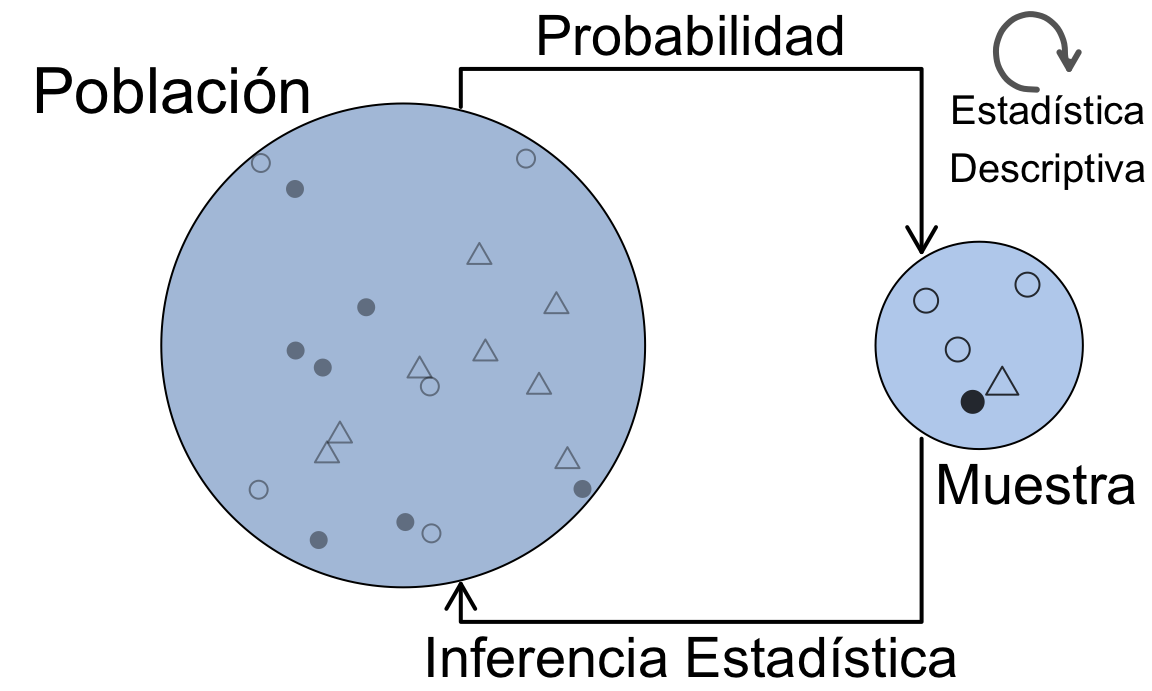
\includegraphics[width=1\linewidth]{images/dogma1} 

}

\caption{La esencia de los métodos estadísticos}\label{fig:dogma1}
\end{figure}

\begin{rmdejemplo}
\includegraphics[width=1em,height=1em]{01-intro_files/figure-latex/fa-icon-37b8d5b2b6c465edf79712060e1bfd05.pdf} En un ensayo clínico, se eligen una serie de participantes en el estudio a los
que se le suministran distintos tratamientos según el diseño del ensayo.
Los participantes en el estudio son sujetos que constituyen la \textbf{muestra}.
A través de los resultados de esta muestra, obtendremos conclusiones
para toda la \textbf{población}, que estará definida en el propio ensayo clínico.
Por ejemplo, en el estudio del efecto de un determinado tratamiento para la
diabetes, la población serían todos los enfermos de diabetes.

\end{rmdejemplo}

Otro concepto clave inherente a la Estadística, es que casi siempre estaremos
investigando sobre esta fórmula:

\[Y=f(X)\]

Es decir, buscamos encontrar la relación entre una variable respuesta \(Y\) y una o varias
variables explicativas \(X\). Casi toda la Ciencia de Datos consiste en encontrar esa \(f\).
Es fundamental interiorizar este concepto para después aplicar el método adecuado,
ya que según sean la/s \(Y\), la/s \(X\) y el objetivo de nuestro estudio, los caminos
pueden ser muy diferentes.

\hypertarget{tipos-de-datos}{%
\section{Tipos de datos}\label{tipos-de-datos}}

Las \textbf{características} que observamos en los \textbf{elementos} de la muestra
(o que estudiamos en una población) pueden ser distintos tipos. Nos referiremos
genéricamente a estas características como \textbf{variables}, aunque en en algunos
ámbitos como el Control Estadístico de Procesos (SPC, \emph{Statistical Process Control}
por sus siglas en inglés) este término se refiere solo a las variables continuas
que ahora definiremos.

Denotaremos las variables con letras mayúsculas del alfabeto latino (\(X\), \(Y\), \(A\), \ldots).
Cuando observamos la característica, la variable toma un \textbf{valor}. Estos valores
pueden ser agrupados en \textbf{clases}, de forma que cada posible valor
pertenezca a una y solo una clase. En ocasiones los datos con los que trabajamos
están ya clasificados en clases.

\begin{rmdejemplo}
Cuando se recogen datos utilizando cuestionarios, a menudo en las preguntas
para recoger características cuantitativas se ofrece elegir un intervalo en vez
de peguntar el \textbf{valor} exacto. Por ejemplo, al preguntar la edad de una
persona, se pueden dar las opciones: 1) menos de 20 años; 2) entre 20 y 40 años;
3) entre 40 y 60 años; 4)Más de 60 años. Así, si una persona tiene 30 años, el \textbf{valor}
de la variable es 30 (en el caso de la encuesta no lo conoceremos exactamente)
que pertenece a la \textbf{clase} ``entre 20 y 40 años''.

\end{rmdejemplo}

Datos univariantes, bivariantes, multivariantes

La importancia de la variabilidad

Calidad y Estadística

Inferencia Estadística y sus técnicas

Ciencia de Datos, Big Data y otras chuches

ODS: algo

\begin{itemize}
\tightlist
\item
  Pueden tomar cualquier valor en su \textbf{dominio} (conjunto de .red{[}\textbf{posibles}{]} valores que puede tomar la variable)
\end{itemize}

--

.media.centrado{[}Siguen una distribución de \textbf{probabilidad}{]}

\begin{longtable}[]{@{}
  >{\raggedright\arraybackslash}p{(\columnwidth - 0\tabcolsep) * \real{0.06}}@{}}
\toprule
\endhead
class: large \\
\#\# Parámetros y Estadísticos \\
.pull-left{[} \\
\#\# Parámetros \\
* Se definen sobre la \textbf{población} \\
* {[}Casi{]} siempre desconocidos \\
* Valores teóricos \\
* Sobre los que haremos inferencia \\
* Letras griegas \\
{]} \\
.pull-right{[} \\
\#\# Estadísticos \\
* Función definida sobre los datos de una \textbf{muestra} (valores de una o más variables) \\
* En cada muestra serán distintos (variabilidad) \\
* Siguen una \textbf{distribución} en el muestreo \\
* Letras latinas \\
{]} \\
\bottomrule
\end{longtable}

class: large
background-image: url(./images/dogma2.png)
background-position: 50\% 50\%
background-size: 75\%

\hypertarget{la-esencia-de-la-estaduxedstica-1}{%
\section{La esencia de la Estadística}\label{la-esencia-de-la-estaduxedstica-1}}

\begin{center}\rule{0.5\linewidth}{0.5pt}\end{center}

class:large
background-image: url(images/tidy\_data.png)
background-position: 50\% 85\%
background-size: 60\%

\hypertarget{organizaciuxf3n-de-los-datos---tidy-data}{%
\section{\texorpdfstring{Organización de los datos - \emph{Tidy data}}{Organización de los datos - Tidy data}}\label{organizaciuxf3n-de-los-datos---tidy-data}}

\begin{itemize}
\item
  Datos rectangulares
\item
  Una columna para cada variable (mismo tipo de datos)
\item
  Una fila para cada observación (elemento, individuo)
\end{itemize}

--

.idea{[}
\includegraphics{./images/idea.png}{]} Analista y software deben entender lo mismo

\begin{center}\rule{0.5\linewidth}{0.5pt}\end{center}

class: large
background-image: url(images/rectangular.png)
background-position: 95\% 50\%
background-size: 45\%

\hypertarget{ejemplo-datos-bien-organizados}{%
\section{Ejemplo: datos bien organizados}\label{ejemplo-datos-bien-organizados}}

.pull-left{[}
- Separar la capa de datos de las capas de presentación y lógica
- Datos para humanos vs datos para máquinas
- El análisis posterior se simplifica si se preparan los datos para la máquina
- Importancia de los .red{[}metadatos{]} (diccionarios de datos){]}

\begin{longtable}[]{@{}
  >{\raggedright\arraybackslash}p{(\columnwidth - 0\tabcolsep) * \real{0.06}}@{}}
\toprule
\endhead
class: large \\
\#\# Tipos de variables \\
* Cuantitativas o Numéricas
+ Continuas
+ Discretas \\
* Cualitativas o Categóricas
+ Multinivel
+ Dicotómicas
+ Ordinales \\
* Marcas de tiempo e identificadores \\
\bottomrule
\end{longtable}

class: large

\hypertarget{escalas}{%
\section{Escalas}\label{escalas}}

\begin{itemize}
\item
  Nominal: atributos, factores, etiquetas
\item
  Ordinal: atributos con un orden lógico
\item
  Métrica: Permiten medir diferencias entre individuos
\end{itemize}

--

\hypertarget{conversiuxf3n}{%
\section{Conversión}\label{conversiuxf3n}}

\begin{itemize}
\tightlist
\item
  Fechas a categóricas (por ejemplo, mes, día de la semana, \ldots)
\item
  Cualitativas a discretas (clases)
\item
  Ordinales como numérica: cuidado, sobre todo si hay pocos datos (\textless100). Mejor
  combinar en índices
\item
  Variables calculadas con otras (por ejemplo, IMC)
\end{itemize}

\begin{center}\rule{0.5\linewidth}{0.5pt}\end{center}

class: large, inverse, toc, middle

\hypertarget{la-estaduxedstica-y-el-muxe9todo-cientuxedfico}{%
\section{2. La Estadística y el método científico}\label{la-estaduxedstica-y-el-muxe9todo-cientuxedfico}}

\begin{center}\rule{0.5\linewidth}{0.5pt}\end{center}

class: large

\hypertarget{bioestaduxedstica}{%
\section{Bioestadística}\label{bioestaduxedstica}}

\hypertarget{la-estaduxedstica-aplicada-a-la-biologuxeda}{%
\section{La Estadística aplicada a la Biología}\label{la-estaduxedstica-aplicada-a-la-biologuxeda}}

\begin{itemize}
\item
  Cualquier análisis de datos, como cualquier disciplina.
\item
  Énfasis en:

  \begin{itemize}
  \tightlist
  \item
    Diseños experimentales
  \item
    Ensayos clínicos
  \item
    Análisis genómico (vínculo con Bioinformática)
  \end{itemize}
\end{itemize}

\begin{longtable}[]{@{}
  >{\raggedright\arraybackslash}p{(\columnwidth - 0\tabcolsep) * \real{0.06}}@{}}
\toprule
\begin{minipage}[b]{\linewidth}\raggedright
class: large
background-image: url(images/mc.jpg)
background-position: 95\% 50\%
background-size: 35\%
\end{minipage} \\
\midrule
\endhead
class: large \\
\#\# 2. Investigación de base \\
* Análisis exploratorio de datos \\
* Identificar relaciones \\
* Posiblemente, cambiar la pregunta del primer paso \\
\bottomrule
\end{longtable}

class: large

\hypertarget{plantear-una-hipuxf3tesis}{%
\section{3. Plantear una hipótesis}\label{plantear-una-hipuxf3tesis}}

\begin{itemize}
\item
  Formalizarla en términos de Hipóteis nula, \(H_0\), e hipótesis alternativa, \(H_1\)
\item
  El planteamiento de la hipótesis determina
  el método estadístico a utilizar, y el diseño
  del experimento (en sentido amplio)
\end{itemize}

\begin{longtable}[]{@{}
  >{\raggedright\arraybackslash}p{(\columnwidth - 0\tabcolsep) * \real{0.06}}@{}}
\toprule
\begin{minipage}[b]{\linewidth}\raggedright
class: large
\end{minipage} \\
\midrule
\endhead
class: large \\
\#\# 5. Analizar resultados y extraer conclusiones \\
* Análisis exploratorio \\
* Contrastes de hipótesis \\
* Validación de los modelos \\
\bottomrule
\end{longtable}

class: large

\hypertarget{comunicar-resultados}{%
\section{6. Comunicar resultados}\label{comunicar-resultados}}

\begin{itemize}
\item
  Informes reproducibles (RMarkdown)
\item
  Gráficos efectivos
\item
  Resultados clave
\item
  Resultados negativos
\end{itemize}

\begin{center}\rule{0.5\linewidth}{0.5pt}\end{center}

class: large, inverse, toc, middle

\hypertarget{estaduxedstica-calidad-y-sostenibilidad}{%
\section{3. Estadística, Calidad y Sostenibilidad}\label{estaduxedstica-calidad-y-sostenibilidad}}

\begin{longtable}[]{@{}
  >{\raggedright\arraybackslash}p{(\columnwidth - 0\tabcolsep) * \real{0.06}}@{}}
\toprule
\begin{minipage}[b]{\linewidth}\raggedright
class: large
\#\# Control Estadístico de la Calidad
\end{minipage} \\
\midrule
\endhead
class: large \\
\#\# Calidad y variabilidad \\
.media{[}
\textgreater{} \textbf{Calidad:} Grado en el que un conjunto de .red{[}características{]} inherentes de un objeto
\textgreater{} cumple con los .red{[}requisitos{]}
\textgreater{}
\textgreater{} ISO 9001:2015 3.6.2 \\
Los requisitos son .red{[}\textbf{especificaciones}{]} de la característica, que pueden ser bilaterales o unilaterales.{]} \\
\bottomrule
\end{longtable}

class: large
background-image: url(images/histos-1.png)
background-position: 50\% 70\%
background-size: 80\%
\#\# La media y la variabilidad

--

Misma media, distinta capacidad de proceso

???

\begin{center}\rule{0.5\linewidth}{0.5pt}\end{center}

class: large
background-image: url(images/taguchi-1.png)
background-position: 50\% 90\%
background-size: 50\%
\#\# Función de pérdida de Taguchi

--

\begin{quote}
La Calidad se mide como la pérdida total que un producto causa a la sociedad

Genichi Taguchi
\end{quote}

???

\begin{longtable}[]{@{}
  >{\raggedright\arraybackslash}p{(\columnwidth - 0\tabcolsep) * \real{0.06}}@{}}
\toprule
\endhead
class: large
background-image: url(images/spc.png)
background-position: 90\% 50\%
background-size: 40\% \\
\#\# SPC: \emph{Statistical Process Control} \\
.pull-left{[}
* Gráficos decontrol \\
* Análisis de la capacidad del proceso \\
* Combinados con otras técnicas estadísticas
{]} \\
\bottomrule
\end{longtable}

class: large
background-image: url(images/qcpass.png)
background-position: 80\% 80\%
background-size: 40\%

\hypertarget{inspecciuxf3n-por-muestreo}{%
\section{Inspección por muestreo}\label{inspecciuxf3n-por-muestreo}}

\begin{itemize}
\item
  AKA Muestreos de aceptación
\item
  Aceptación: dentro de los límites de especificación
\item
  Por atributos y por variables
\item
  La base: probabilidad de aceptar/rechazar un lote defectuoso/correcto
\item
  Muestreos por lotes
\item
  Planes simples
\item
  Planes dobles y múltiples
\item
  Planes secuenciales
\item
  MIL-STD -\textgreater{} ISO 2859
\end{itemize}

\begin{longtable}[]{@{}
  >{\raggedright\arraybackslash}p{(\columnwidth - 0\tabcolsep) * \real{0.06}}@{}}
\toprule
\begin{minipage}[b]{\linewidth}\raggedright
class: large
background-image: url(images/micro.jpg)
background-position: 90\% 90\%
background-size: 35\%
\#\# Ensayos inter-laboratorios
\end{minipage} \\
\midrule
\endhead
class: large \\
\#\# Metodologías y estándares \\
* ISO TC69 + UNE CT66/SC3 \\
* Metodología Seis Sigma y el ciclo DMAIC \\
* Lean Six Sigma \\
* ISO 9000 + UNE-ISO TR 1017 (Orientación sobre las técnicas estadísticas para la Norma ISO 9001:2020) \\
.idea{[}
\includegraphics{images/idea.png} En la biblioteca de la URJC tenéis disponible la coleccción de normas UNE{]} \\
\bottomrule
\end{longtable}

class: huge

\hypertarget{objetivos-de-desarrollo-sostenible-ods}{%
\section{Objetivos de Desarrollo Sostenible (ODS)}\label{objetivos-de-desarrollo-sostenible-ods}}

\begin{itemize}
\tightlist
\item
  Iniciativa de la ONU: \emph{Sustainable Development Goals} (SDG)
\item
  17 objetivos
\item
  169 metas
\end{itemize}

\begin{quote}
El 25 de septiembre de 2015, los líderes mundiales adoptaron un conjunto de .red{[}\textbf{objetivos globales}{]} para erradicar la pobreza, proteger el planeta y asegurar la prosperidad para todos como parte de una nueva agenda de desarrollo sostenible. Cada objetivo tiene .red{[}\textbf{metas específicas}{]} que deben alcanzarse en los próximos 15 años.

\href{https://www.un.org/sustainabledevelopment/es/objetivos-de-desarrollo-sostenible/}{Naciones Unidas}
\end{quote}

class: large
background-image: url(./images/nature.jpg)
background-position: 90\% 90\%
background-size: 25\%

\hypertarget{bioestaduxedstica-y-sostenibilidad}{%
\section{Bioestadística y sostenibilidad}\label{bioestaduxedstica-y-sostenibilidad}}

\begin{itemize}
\item
  Analizar datos relacionados con los ODS (Investigar)
\item
  Ser sostenible en los análisis
\item
  Relacionar con ODS e intentar contribuir sea cual sea el objetivo de la
  investigación
\item
  ¿Cómo puede contribuir este trabajo/estudio/investigación/\ldots{}\\
  a conseguir los Objetivos de Desarrollo Sostenible?
\end{itemize}

\hypertarget{aed-uni}{%
\chapter{Análisis exploratorio univariante}\label{aed-uni}}

Resúmenes numéricos

Resúmenes gráficos

Valores atípicos

Valores perdidos

En preparación.

\hypertarget{aed-bi}{%
\chapter{Análisis exploratorio bivariante}\label{aed-bi}}

Representación gráfica

Correlación

Regresión

Intro multivariante

En preparación.

\hypertarget{part-probabilidad}{%
\part{Probabilidad}\label{part-probabilidad}}

\hypertarget{introp}{%
\chapter{Introducción a la Probabilidad}\label{introp}}

En preparación.

Definiciones

Propiedades

Probabilidad total y Bayes

\hypertarget{vauni}{%
\chapter{Variable aleatoria univariante}\label{vauni}}

En preparación.

Definición

Función de distribución

VA discreta

VA continua

\hypertarget{vabi}{%
\chapter{Variable aleatoria bivariante}\label{vabi}}

En preparación.

Distribución conjunta

Correlación y regresión

\hypertarget{modelos}{%
\chapter{Modelos de distribución de probabilidad}\label{modelos}}

En preparación.

Introducción

Modelos discretos

Modelos continuos

Modelos multivariantes*

\hypertarget{part-inferencia-estaduxedstica}{%
\part{Inferencia estadística}\label{part-inferencia-estaduxedstica}}

\hypertarget{muestreo}{%
\chapter{Muestreo y estimación}\label{muestreo}}

En preparación.

Muestreo estadístico

Estimación y contrastes

Estadísticos

Estimadores puntuales (medias, proporciones, varianzas)

Estimación por intervalos

Estimación no paramétrica

Inferencia Bayesiana*

\hypertarget{comparacion}{%
\chapter{Comparación de grupos}\label{comparacion}}

En preparación.

Comparación de atributos

Comparación de dos grupos

Comparación de más de dos grupos

\hypertarget{regresion}{%
\chapter{Modelos de regresión}\label{regresion}}

En preparación.

Regresión lineal simple

Regresión no lineal

Regresión lineal múltiple

Otros modelos*\\
(GLM, GAM, \ldots)

\hypertarget{doe}{%
\chapter{Diseño de experimentos}\label{doe}}

En preparación.

Intro

Diseños factoriales

Diseños \(2^k\)

Diseños fraccionales

\hypertarget{part-control-estaduxedstico-de-la-calidad}{%
\part{Control estadístico de la calidad}\label{part-control-estaduxedstico-de-la-calidad}}

\hypertarget{introc}{%
\chapter{Introducción}\label{introc}}

En preparación.

Historia de la calidad

Estadística y calidad

Gestión de la calidad

Mejora de procesos vs control de calidad

Metodologías

Intro Six Sigma*

\hypertarget{spc}{%
\chapter{Control Estadístico de Procesos}\label{spc}}

En preparación.

Intro SPC

Gráficos de control

Capacidad y rendimiento

\hypertarget{aceptacion}{%
\chapter{Inspección por muestreo}\label{aceptacion}}

En preparación.

Intro

Planes para atributos

Planes para variables

\hypertarget{appendix-apuxe9ndices}{%
\appendix}


\hypertarget{suxedmbolos-abreviaturas-y-acruxf3nimos}{%
\chapter{Símbolos, abreviaturas y acrónimos}\label{suxedmbolos-abreviaturas-y-acruxf3nimos}}

\hypertarget{acruxf3nimos}{%
\section{Acrónimos}\label{acruxf3nimos}}

\begin{longtable}[]{@{}ll@{}}
\toprule
Acrónimo & Descripción \\
\midrule
\endhead
SPC & Statistical Process Control \\
\bottomrule
\end{longtable}

\hypertarget{letras-griegas}{%
\section{Letras griegas}\label{letras-griegas}}

\begin{longtable}[]{@{}ll@{}}
\toprule
Letra & Se lee \\
\midrule
\endhead
\(\alpha\) & alfa \\
\(\beta\) & beta \\
\(\gamma\) & gamma \\
\(\Gamma\) & Gamma\(^*\) \\
\(\lambda\) & lambda \\
\(\eta\) & eta \\
\(\mu\) & mu \\
\(\omega\) & omega \\
\(\Omega\) & Omega\(^*\) \\
\(\sigma\) & sigma \\
\(\Sigma\) & Sigma\(^*\) \\
\(\rho\) & ro \\
\(\theta\) & zeta (\emph{theta}, teta) \\
\(\xi\) & xi \\
\(\chi\) & chi (o \emph{ji}) \\
\(\pi\) & pi \\
\(\varepsilon\) & épsilon \\
\bottomrule
\end{longtable}

\(^*\) Mayúsculas

\hypertarget{suxedmbolos}{%
\section{Símbolos}\label{suxedmbolos}}

\begin{longtable}[]{@{}ll@{}}
\toprule
Símbolo & Se lee \\
\midrule
\endhead
\(\emptyset\) & Conjunto vacío o suceso imposible \\
\(\aleph\) & Aleph \\
\(\wp\) & Probabilidad (como función) \\
\(:\) & Tal que \\
\(P(\cdot)\) & Probabilidad de · (sucesos) \\
\(P[\cdot]\) & Probabilidad de · (variables aleatorias) \\
\(E[\cdot]\) & Esperanza de · \\
\(\cdot\) & \emph{lo que sea} (representa cualquier objeto matemático) \\
\(|\) & Condicionado a \\
\(\sum\) & Sumatorio \\
\(\sum\limits_{i=1}^n\) & Sumatorio desde \(i\) igual a uno hasta \(n\) \\
\(\prod\) & Producto \\
\(\prod\limits_{i=1}^n\) & Producto desde \(i\) igual a uno hasta \(n\) \\
\(\forall\) & Para todo \\
\(\in\) & Pertenece/perteneciente \\
\(\exists\) & Existe \\
\(\implies\) & Implica/entonces \\
\(\partial\) & Derivada parcial \\
\(\simeq\) & Aproximadamente igual\footnote{En este libro se usa sobre todo para indicar que se ha redondeado un número decimal} \\
\(\approx\) & Aproximadamente\footnote{En este libro se puede utilizar para tomar el entero superior o inferior según el contexto} \\
\(\equiv\) & Equivalente \\
\(\mathbb{R}\) & Conjunto de los números reales \\
\(\cup\) & Unión \\
\(\cap\) & Intersección \\
\(\subset\) & Incluido \\
\(\subseteq\) & Incluido o igual \\
\bottomrule
\end{longtable}

\hypertarget{tablas}{%
\chapter{Tablas estadísticas}\label{tablas}}

\hypertarget{distribuciuxf3n-normal}{%
\section{Distribución normal}\label{distribuciuxf3n-normal}}

La siguiente tabla contiene la probabilidad de la cola superior de la distribución normal estándar \(Z\sim N(0;1)\),
es decir \(1-F(z)=P[Z>z].\).

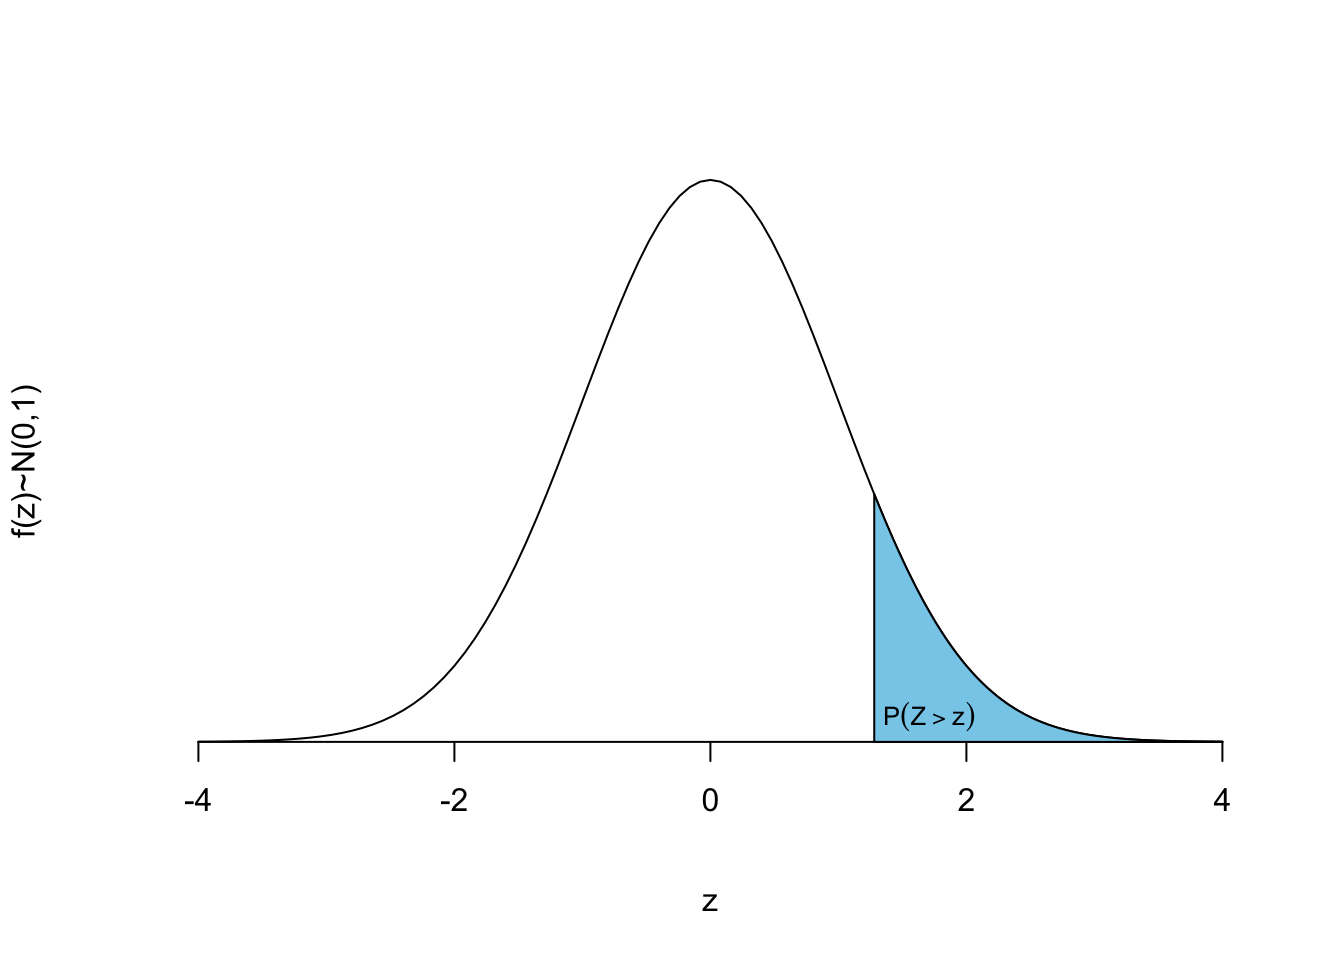
\includegraphics[width=0.7\linewidth]{91-apendices_files/figure-latex/unnamed-chunk-2-1}

\begin{tabular}{r|r|r|r|r|r|r|r|r|r|r}
\hline
z & 0.00 & 0.01 & 0.02 & 0.03 & 0.04 & 0.05 & 0.06 & 0.07 & 0.08 & 0.09\\
\hline
0.0 & 0.5000 & 0.4960 & 0.4920 & 0.4880 & 0.4840 & 0.4801 & 0.4761 & 0.4721 & 0.4681 & 0.4641\\
\hline
0.1 & 0.4602 & 0.4562 & 0.4522 & 0.4483 & 0.4443 & 0.4404 & 0.4364 & 0.4325 & 0.4286 & 0.4247\\
\hline
0.2 & 0.4207 & 0.4168 & 0.4129 & 0.4090 & 0.4052 & 0.4013 & 0.3974 & 0.3936 & 0.3897 & 0.3859\\
\hline
0.3 & 0.3821 & 0.3783 & 0.3745 & 0.3707 & 0.3669 & 0.3632 & 0.3594 & 0.3557 & 0.3520 & 0.3483\\
\hline
0.4 & 0.3446 & 0.3409 & 0.3372 & 0.3336 & 0.3300 & 0.3264 & 0.3228 & 0.3192 & 0.3156 & 0.3121\\
\hline
0.5 & 0.3085 & 0.3050 & 0.3015 & 0.2981 & 0.2946 & 0.2912 & 0.2877 & 0.2843 & 0.2810 & 0.2776\\
\hline
0.6 & 0.2743 & 0.2709 & 0.2676 & 0.2643 & 0.2611 & 0.2578 & 0.2546 & 0.2514 & 0.2483 & 0.2451\\
\hline
0.7 & 0.2420 & 0.2389 & 0.2358 & 0.2327 & 0.2296 & 0.2266 & 0.2236 & 0.2206 & 0.2177 & 0.2148\\
\hline
0.8 & 0.2119 & 0.2090 & 0.2061 & 0.2033 & 0.2005 & 0.1977 & 0.1949 & 0.1922 & 0.1894 & 0.1867\\
\hline
0.9 & 0.1841 & 0.1814 & 0.1788 & 0.1762 & 0.1736 & 0.1711 & 0.1685 & 0.1660 & 0.1635 & 0.1611\\
\hline
1.0 & 0.1587 & 0.1562 & 0.1539 & 0.1515 & 0.1492 & 0.1469 & 0.1446 & 0.1423 & 0.1401 & 0.1379\\
\hline
1.1 & 0.1357 & 0.1335 & 0.1314 & 0.1292 & 0.1271 & 0.1251 & 0.1230 & 0.1210 & 0.1190 & 0.1170\\
\hline
1.2 & 0.1151 & 0.1131 & 0.1112 & 0.1093 & 0.1075 & 0.1056 & 0.1038 & 0.1020 & 0.1003 & 0.0985\\
\hline
1.3 & 0.0968 & 0.0951 & 0.0934 & 0.0918 & 0.0901 & 0.0885 & 0.0869 & 0.0853 & 0.0838 & 0.0823\\
\hline
1.4 & 0.0808 & 0.0793 & 0.0778 & 0.0764 & 0.0749 & 0.0735 & 0.0721 & 0.0708 & 0.0694 & 0.0681\\
\hline
1.5 & 0.0668 & 0.0655 & 0.0643 & 0.0630 & 0.0618 & 0.0606 & 0.0594 & 0.0582 & 0.0571 & 0.0559\\
\hline
1.6 & 0.0548 & 0.0537 & 0.0526 & 0.0516 & 0.0505 & 0.0495 & 0.0485 & 0.0475 & 0.0465 & 0.0455\\
\hline
1.7 & 0.0446 & 0.0436 & 0.0427 & 0.0418 & 0.0409 & 0.0401 & 0.0392 & 0.0384 & 0.0375 & 0.0367\\
\hline
1.8 & 0.0359 & 0.0351 & 0.0344 & 0.0336 & 0.0329 & 0.0322 & 0.0314 & 0.0307 & 0.0301 & 0.0294\\
\hline
1.9 & 0.0287 & 0.0281 & 0.0274 & 0.0268 & 0.0262 & 0.0256 & 0.0250 & 0.0244 & 0.0239 & 0.0233\\
\hline
2.0 & 0.0228 & 0.0222 & 0.0217 & 0.0212 & 0.0207 & 0.0202 & 0.0197 & 0.0192 & 0.0188 & 0.0183\\
\hline
2.1 & 0.0179 & 0.0174 & 0.0170 & 0.0166 & 0.0162 & 0.0158 & 0.0154 & 0.0150 & 0.0146 & 0.0143\\
\hline
2.2 & 0.0139 & 0.0136 & 0.0132 & 0.0129 & 0.0125 & 0.0122 & 0.0119 & 0.0116 & 0.0113 & 0.0110\\
\hline
2.3 & 0.0107 & 0.0104 & 0.0102 & 0.0099 & 0.0096 & 0.0094 & 0.0091 & 0.0089 & 0.0087 & 0.0084\\
\hline
2.4 & 0.0082 & 0.0080 & 0.0078 & 0.0075 & 0.0073 & 0.0071 & 0.0069 & 0.0068 & 0.0066 & 0.0064\\
\hline
2.5 & 0.0062 & 0.0060 & 0.0059 & 0.0057 & 0.0055 & 0.0054 & 0.0052 & 0.0051 & 0.0049 & 0.0048\\
\hline
2.6 & 0.0047 & 0.0045 & 0.0044 & 0.0043 & 0.0041 & 0.0040 & 0.0039 & 0.0038 & 0.0037 & 0.0036\\
\hline
2.7 & 0.0035 & 0.0034 & 0.0033 & 0.0032 & 0.0031 & 0.0030 & 0.0029 & 0.0028 & 0.0027 & 0.0026\\
\hline
2.8 & 0.0026 & 0.0025 & 0.0024 & 0.0023 & 0.0023 & 0.0022 & 0.0021 & 0.0021 & 0.0020 & 0.0019\\
\hline
2.9 & 0.0019 & 0.0018 & 0.0018 & 0.0017 & 0.0016 & 0.0016 & 0.0015 & 0.0015 & 0.0014 & 0.0014\\
\hline
3.0 & 0.0013 & 0.0013 & 0.0013 & 0.0012 & 0.0012 & 0.0011 & 0.0011 & 0.0011 & 0.0010 & 0.0010\\
\hline
3.1 & 0.0010 & 0.0009 & 0.0009 & 0.0009 & 0.0008 & 0.0008 & 0.0008 & 0.0008 & 0.0007 & 0.0007\\
\hline
3.2 & 0.0007 & 0.0007 & 0.0006 & 0.0006 & 0.0006 & 0.0006 & 0.0006 & 0.0005 & 0.0005 & 0.0005\\
\hline
3.3 & 0.0005 & 0.0005 & 0.0005 & 0.0004 & 0.0004 & 0.0004 & 0.0004 & 0.0004 & 0.0004 & 0.0003\\
\hline
3.4 & 0.0003 & 0.0003 & 0.0003 & 0.0003 & 0.0003 & 0.0003 & 0.0003 & 0.0003 & 0.0003 & 0.0002\\
\hline
3.5 & 0.0002 & 0.0002 & 0.0002 & 0.0002 & 0.0002 & 0.0002 & 0.0002 & 0.0002 & 0.0002 & 0.0002\\
\hline
3.6 & 0.0002 & 0.0002 & 0.0001 & 0.0001 & 0.0001 & 0.0001 & 0.0001 & 0.0001 & 0.0001 & 0.0001\\
\hline
3.7 & 0.0001 & 0.0001 & 0.0001 & 0.0001 & 0.0001 & 0.0001 & 0.0001 & 0.0001 & 0.0001 & 0.0001\\
\hline
3.8 & 0.0001 & 0.0001 & 0.0001 & 0.0001 & 0.0001 & 0.0001 & 0.0001 & 0.0001 & 0.0001 & 0.0001\\
\hline
3.9 & 0.0000 & 0.0000 & 0.0000 & 0.0000 & 0.0000 & 0.0000 & 0.0000 & 0.0000 & 0.0000 & 0.0000\\
\hline
\end{tabular}

\hypertarget{resumen-modelos-de-distribuciuxf3n-de-probabilidad}{%
\section{Resumen modelos de distribución de probabilidad}\label{resumen-modelos-de-distribuciuxf3n-de-probabilidad}}

\begin{tabular}{l|l|l|l}
\hline
Distribución & Probabilidad/Densidad/Distribución & Esperanza & Varianza\\
\hline
\$\textbackslash{}text\{Bernoulli\}\textbackslash{}\textbackslash{} \textbackslash{}mathit\{Ber\}(p)\$ & \$X = \textbackslash{}begin\{cases\} 1 \& \textbackslash{}mbox\{ con probabilidad \} p \textbackslash{}\textbackslash{} 0 \& \textbackslash{}mbox\{ con probabilidad \} 1-p \textbackslash{}end\{cases\}\$ & \$p\$ & \$p(1-p)\$\\
\hline
\end{tabular}

\hypertarget{repaso}{%
\chapter{Repaso}\label{repaso}}

Este apéndice cubre algunas cuestiones matemáticas básicas que el lector
de este libro con seguridad habrá aprendido con anterioridad. Se incluyen
como referencia para facilitar el repaso a aquellos que lo necesiten.

\hypertarget{logaritmos-y-exponenciales}{%
\section{Logaritmos y exponenciales}\label{logaritmos-y-exponenciales}}

\hypertarget{combinatoria}{%
\section{Combinatoria}\label{combinatoria}}

Una de las definiciones de probabilidad implica \textbf{contar}
el número de veces que puede ocurrir un suceso determinado. Por tanto,
en muchas ocasiones el cálculo de probabilidades empieza contando las
posibilidades de que ocurra un suceso. La Combinatoria es la parte de la
Matemática discreta que nos ayuda en esta tarea. Incluimos un breve
resumen con ejemplos de las fórmulas más habituales y su cálculo con R.

\hypertarget{ejemplo-ilustrativo}{%
\subsection{Ejemplo ilustrativo}\label{ejemplo-ilustrativo}}

Habitualmente se utilizan ejemplos de juegos de azar para introducir el
cálculo de probabilidades, como lanzamiendo de monedas y dados, o
combinaciones de cartas en barajas de naipes. Para darle un enfoque
práctico, utilizaremos a lo largo del módulo un ejemplo ilustrativo que,
aunque totalmente inventado, se puede encontrar el lector
en el futuro con ligeras variaciones según su ámbito de actuación.
Utilizaremos en lo posible las cifras usadas en los problemas de azar
para ver la utilidad de aquéllos ejemplos en casos más prácticos.

Datos básicos:

\begin{itemize}
\item
  52 posibles usuarios de un servicio
\item
  La mitad son mujeres
\item
  4 directivos, 12 mandos, resto operarios
\item
  13 jóvenes, 26 adultos, 13 mayores (5, 18 y 3 mujeres en cada
  grupo respectivamente)
\item
  1 de cada seis hombres contratará el servicio (el doble si es mujer)
\end{itemize}

Nótese cómo podemos \emph{traducir} el concepto de
servicio a cualquier ámbito: usuarios de salud o educación, enfermos de
una determinada patología, equipos de una infraestructura, etc. Asimismo
las categorías pueden ser cualesquiera aplicables a los elementos de los
conjuntos.

\hypertarget{principio-buxe1sico-de-conteo}{%
\subsection{Principio básico de conteo}\label{principio-buxe1sico-de-conteo}}

\textbf{Definición}: Realizamos \(k\) experimentos sucesivamente, cada
uno de ellos con \(n_i\) posibles resultados (\(i=1, \ldots, k\)). Entonces
el número total de resultados posibles es:

\[n_1\cdot n_2, \cdot \ldots \cdot n_k\]

\textbf{Ejemplo}: Resultados posibles si tomamos al azar un individuo
y observamos su grupo de edad y si contratará o no el servicio.

\textbf{Código}

\begin{Shaded}
\begin{Highlighting}[]
\DecValTok{3}\SpecialCharTok{*}\DecValTok{2}
\CommentTok{\#\textgreater{} [1] 6}
\end{Highlighting}
\end{Shaded}

\hypertarget{permutaciones}{%
\subsection{Permutaciones}\label{permutaciones}}

\textbf{Definición}: De cuántas formas posibles podemos ordenar un
conjunto de \(n\) elementos sin repetirlos.

\[P_n = n! = n\cdot(n-1)\cdot(n-2)\cdot\ldots\cdot 2\cdot 1\]

\textbf{Ejemplo}: De cuántas formas podemos ordenar un conjunto de
tres individuos, uno de cada categoría laboral.

\textbf{Código}

\begin{Shaded}
\begin{Highlighting}[]
\FunctionTok{factorial}\NormalTok{(}\DecValTok{3}\NormalTok{)}
\CommentTok{\#\textgreater{} [1] 6}
\end{Highlighting}
\end{Shaded}

\hypertarget{variaciones-muestreo-sin-reemplazamiento}{%
\subsection{Variaciones (muestreo sin reemplazamiento)}\label{variaciones-muestreo-sin-reemplazamiento}}

\textbf{Definición}: De cuántas formas posibles podemos seleccionar
una muestra de \(n\) elementos de un conjunto total de \(m\), sin que se
repitan. Una ordenación distinta, es una posibilidad distinta.

\[V_{m,n} = m\cdot(m-1)\cdot(m-2)\cdot\ldots\cdot (m-n+1) = \frac{m!}{(m-n)!}\]

\textbf{Ejemplo}: De cuántas formas podemos seleccionar una muestra
de 5 individuos en nuestro conjunto de 52 sin que se repitan (por
ejemplo para asignar un ranking)

\textbf{Código}

\begin{Shaded}
\begin{Highlighting}[]
\FunctionTok{factorial}\NormalTok{(}\DecValTok{52}\NormalTok{)}\SpecialCharTok{/}\FunctionTok{factorial}\NormalTok{(}\DecValTok{52{-}5}\NormalTok{)}
\CommentTok{\#\textgreater{} [1] 311875200}
\end{Highlighting}
\end{Shaded}

\hypertarget{variaciones-con-repeticiuxf3n-muestreo-con-reemplazamiento}{%
\subsection{Variaciones con repetición (muestreo con reemplazamiento)}\label{variaciones-con-repeticiuxf3n-muestreo-con-reemplazamiento}}

\textbf{Definición}: De cuántas formas posibles podemos seleccionar
una muestra de \(n\) elementos de un conjunto total de \(m\), pudiéndose
repetir. Una ordenación distinta, es una posibilidad distinta.
\[\mathit{VR}_{m,n} = m^n\]

\textbf{Ejemplo}: De cuántas formas podemos seleccionar una muestra
de 5 individuos en nuestro conjunto de 52 pudiéndose repetir (por
ejemplo para asignar premios consecutivamente)

\textbf{Código}

\begin{Shaded}
\begin{Highlighting}[]
\DecValTok{52}\SpecialCharTok{\^{}}\DecValTok{5}
\CommentTok{\#\textgreater{} [1] 380204032}
\end{Highlighting}
\end{Shaded}

\hypertarget{combinaciones-muestras-equivalentes}{%
\subsection{Combinaciones (muestras equivalentes)}\label{combinaciones-muestras-equivalentes}}

\textbf{Definición}: De cuántas formas posibles podemos seleccionar
una muestra de \(n\) elementos de un conjunto total de \(m\), sin importar
el orden.

\[\mathit{C}_{m,n} = \binom{m}{n} = \frac{m!}{n!(m-n)!}\]

\(\binom{m}{n}\) se lee \emph{m sobre n}, y se le conoce como \emph{número combinatorio}.
Algunas propiedades importantes de los números combinatorios:

\[\binom{m}{m} = \binom{m}{0} = 1.\]
\[\binom{m}{1} = \binom{m}{m-1} = m.\]
\[\binom{m}{n} + \binom{m}{n+1} = \binom{m+1}{n+1}\]
Por otra parte, por convenio se tiene que:

\[0!=1,\]

\[\text{si } a <b \implies \binom{a}{b} = 0.\]

\textbf{Ejemplo}: De cuántas formas podemos seleccionar una muestra
de 5 individuos en nuestro conjunto de 52 sin importar el orden (por
ejemplo para asignar premios de una sola vez)

\textbf{Código}

\begin{Shaded}
\begin{Highlighting}[]
\FunctionTok{choose}\NormalTok{(}\DecValTok{52}\NormalTok{, }\DecValTok{5}\NormalTok{)}
\CommentTok{\#\textgreater{} [1] 2598960}
\end{Highlighting}
\end{Shaded}

\hypertarget{combinaciones-y-permutaciones-con-repeticiuxf3n}{%
\subsection{Combinaciones y permutaciones con repetición}\label{combinaciones-y-permutaciones-con-repeticiuxf3n}}

Las combinaciones y
permutaciones también se pueden dar con repetición, siendo las fórmulas
para calcularlas las siguientes:

\[\mathit{CR}_{m,n}= \mathit{C}_{m+n-1,n}= \frac{(m+n-1)!}{n!\cdot(m-1)!}\]
\[\mathit{PR} = \frac{n!}{a!\cdot b!\cdot \ldots\cdot z!}\]

La primera situación es aquella en la que los
elementos se pueden repetir, pero no nos importa el orden en que lo
hagan. La segunda aparece cuando el elemento A del conjunto total de
elementos aparece \(a\) veces, y así sucesivamente.

\hypertarget{ampliaciuxf3n}{%
\chapter{Ampliación}\label{ampliaciuxf3n}}

En este apéndice se incluyen temas avanzados que pueden ser útiles al lector
más allá de un curso básico de estadística para ciencias o ingeniería, y
que no se han incluido en el cuerpo de los capítulos para mantener el nivel
de una asignatura de grado.

\hypertarget{funciuxf3n-caracteruxedstica}{%
\section{Función característica}\label{funciuxf3n-caracteruxedstica}}

\hypertarget{cambio-de-variable}{%
\section{Cambio de variable}\label{cambio-de-variable}}

\hypertarget{variables-aleatorias-unidimensionales-mixtas}{%
\section{Variables aleatorias unidimensionales mixtas}\label{variables-aleatorias-unidimensionales-mixtas}}

\hypertarget{variables-aleatorias-bidimensionales-mixtas}{%
\section{Variables aleatorias bidimensionales mixtas}\label{variables-aleatorias-bidimensionales-mixtas}}

\hypertarget{algunos-modelos-de-distribuciuxf3n-continuos-muxe1s}{%
\section{Algunos modelos de distribución continuos más}\label{algunos-modelos-de-distribuciuxf3n-continuos-muxe1s}}

\hypertarget{distribuciuxf3n-beta}{%
\subsection{Distribución Beta}\label{distribuciuxf3n-beta}}

La distribución Beta se utiliza en problemas de inferencia relativos a proporciones, especialmente en inferencia bayesiana.

\[X \sim \mathit{Be}(\alpha, \beta)\]

\textbf{Función de densidad}

\[f(x) = 
\begin{cases}
\frac{\Gamma(\alpha + \beta)}{\Gamma(\alpha)\Gamma(\beta)}x^{\alpha-1}(1-x)^{\beta -1} & \text{si } 0 < x < 1\\
0 & \text{resto } 
\end{cases}\]

En matemáticas, la función Gamma (\(\Gamma\)) es una integral indefinida que tiene entre otras las siguientes propiedades:

\begin{itemize}
\tightlist
\item
  \$\Gamma(\alpha) = \int\_0\textsuperscript{\infty x}\{\alpha -1\} e\^{}\{-x\} dx, \qquad \alpha \textgreater{} 0 \$
\item
  \(\Gamma(\alpha + 1) = \alpha \Gamma(\alpha)\)
\item
  \(n \in \mathbb{N}-\{0\} \implies \Gamma(n) = (n-1)!\)
\item
  \(\Gamma(\frac{1}{2}) = \sqrt{\pi}\)
\end{itemize}

** Características**

\begin{itemize}
\tightlist
\item
  Esperanza: \(E[X] = \frac{\alpha}{\alpha + \beta}\)
\item
  Varianza: \(\mathit{Var}[X] = \frac{\alpha\beta}{(\alpha + \beta)^2(\alpha + \beta+1)}\)
\item
  Caso particular: \(\mathit{Be}(1,1) = U(0,1)\).
\end{itemize}

\textbf{Ejemplo}

\(X\): Proporción de clientes que contratarán el servicio

\(X\sim \mathit{Be}(1, 5)\)

\textbf{Código}

\begin{Shaded}
\begin{Highlighting}[]
\NormalTok{mibeta }\OtherTok{\textless{}{-}} \ControlFlowTok{function}\NormalTok{(x) }\FunctionTok{dbeta}\NormalTok{(x, }\DecValTok{1}\NormalTok{, }\DecValTok{5}\NormalTok{)}
\FunctionTok{curve}\NormalTok{(mibeta, }\AttributeTok{lwd =} \DecValTok{2}\NormalTok{)}
\end{Highlighting}
\end{Shaded}

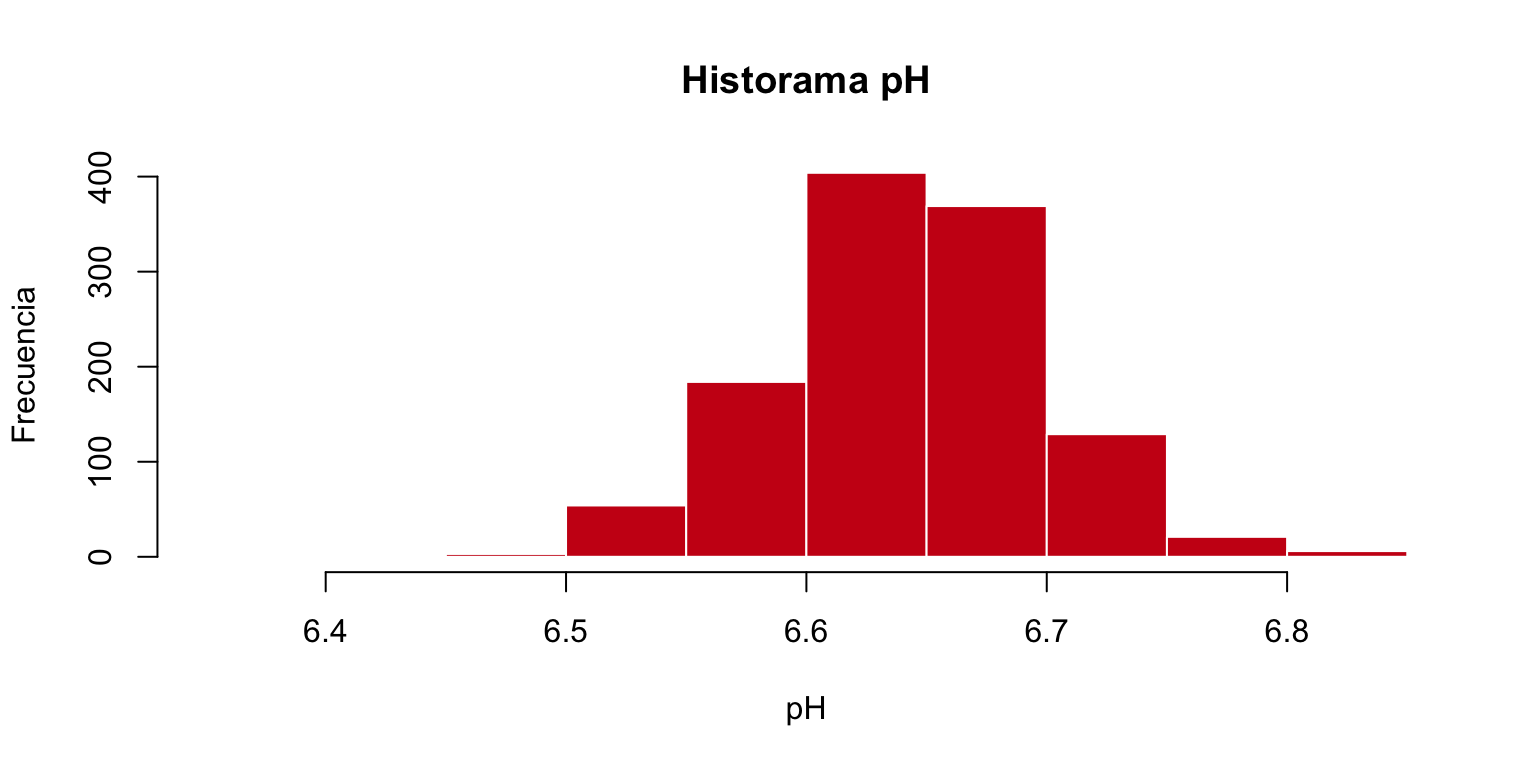
\includegraphics{91-apendices_files/figure-latex/unnamed-chunk-10-1.pdf}

\hypertarget{distribuciuxf3n-gamma}{%
\subsection{Distribución Gamma}\label{distribuciuxf3n-gamma}}

La distribución Gamma se utiliza, entre otros, para modelizar tiempos de espera hasta que suceden \(\alpha\) eventos en un proceso de Poisson. De hecho, en inferencia bayesiana gamma es la distribución a priori de la distribución de Poisson.

\[X \sim \mathit{Ga}(a, b)\]

\textbf{Función de densidad}

\[f(x) =
\begin{cases}
\frac{b^a}{\Gamma(a)}x^{a-1}{e}^{-bx} & \text{si } 0 < x < \infty\\
0 & \text{resto }
\end{cases}\]

\textbf{Características}

\begin{itemize}
\tightlist
\item
  Esperanza: \(E[X] = \frac{a}{b}\)
\item
  Varianza: \(\mathit{Var}[X] = \frac{a}{b^2}\)
\item
  \$\Gamma(\alpha) = \int\_0\textsuperscript{\infty x}\{\alpha -1\} e\^{}\{-x\} dx \$
\item
  La exponencial es un caso particular
\end{itemize}

\textbf{Código}

\begin{Shaded}
\begin{Highlighting}[]
\NormalTok{migamma }\OtherTok{\textless{}{-}} \ControlFlowTok{function}\NormalTok{(x, a) }\FunctionTok{dgamma}\NormalTok{(x, a, }\DecValTok{2}\NormalTok{)}
\FunctionTok{curve}\NormalTok{(}\FunctionTok{migamma}\NormalTok{(x, }\DecValTok{1}\NormalTok{), }\AttributeTok{lwd =} \DecValTok{2}\NormalTok{, }\AttributeTok{xlim =} \FunctionTok{c}\NormalTok{(}\DecValTok{0}\NormalTok{,}\DecValTok{10}\NormalTok{), }
      \AttributeTok{main =} \StringTok{"Distribución Gamma b = 2"}\NormalTok{)}
\FunctionTok{curve}\NormalTok{(}\FunctionTok{migamma}\NormalTok{(x, }\DecValTok{2}\NormalTok{), }\AttributeTok{lwd =} \DecValTok{2}\NormalTok{, }\AttributeTok{add =} \ConstantTok{TRUE}\NormalTok{, }\AttributeTok{lty =} \DecValTok{2}\NormalTok{)}
\FunctionTok{curve}\NormalTok{(}\FunctionTok{migamma}\NormalTok{(x, }\DecValTok{4}\NormalTok{), }\AttributeTok{lwd =} \DecValTok{2}\NormalTok{, }\AttributeTok{add =} \ConstantTok{TRUE}\NormalTok{, }\AttributeTok{lty =} \DecValTok{3}\NormalTok{)}
\FunctionTok{legend}\NormalTok{(}\AttributeTok{x =} \DecValTok{6}\NormalTok{, }\AttributeTok{y =} \DecValTok{2}\NormalTok{, }\FunctionTok{c}\NormalTok{(}\StringTok{"a = 1"}\NormalTok{, }\StringTok{"a = 2"}\NormalTok{, }\StringTok{"a = 4"}\NormalTok{), }\AttributeTok{lty =} \DecValTok{1}\SpecialCharTok{:}\DecValTok{3}\NormalTok{)}
\end{Highlighting}
\end{Shaded}

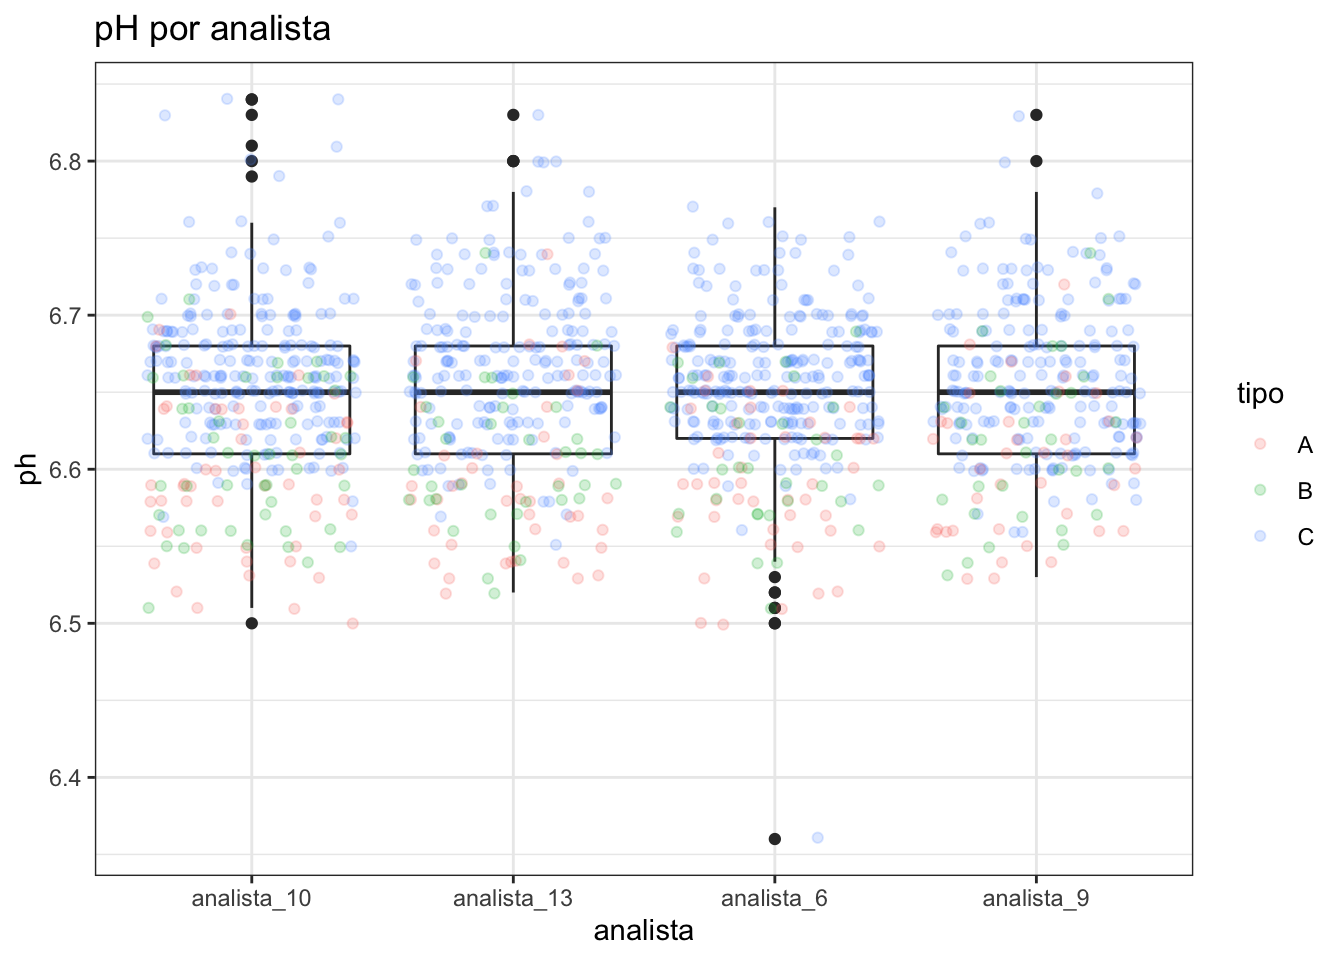
\includegraphics{91-apendices_files/figure-latex/unnamed-chunk-11-1.pdf}

\hypertarget{distribuciuxf3n-de-weibull}{%
\subsection{Distribución de Weibull}\label{distribuciuxf3n-de-weibull}}

La distribución Gamma presenta algunos inconventientes al modelizar tiempos de vida, y por eso algunas veces se prefiere la distribución de Weibull, que básicamente sirve para lo mismo. Véase \cite{ugarte2015} para los detalles.

\[X \sim \mathit{We}(a, b) \]

\textbf{Función de densidad}
\[f(x) =
\begin{cases}
\frac{a}{b}\left (\frac{x}{b} \right)^{a-1}e^{-(x/b)^a} & \text{si } x > 0\\
0 & \text{resto }
\end{cases}\]

\textbf{Características}

\begin{itemize}
\tightlist
\item
  Esperanza: \(E[X] =b \Gamma\left (1 + \frac{1}{a} \right )\)
\item
  Varianza: \(\mathit{Var}[X] = b^2 \left ( \Gamma \left (  1 + \frac{2}{a} \right  )  - \left ( \Gamma \left (1 + \frac{2}{a} \right ) \right )^2 \right )\)
\end{itemize}

\textbf{Código}

\begin{Shaded}
\begin{Highlighting}[]
\NormalTok{miweibull }\OtherTok{\textless{}{-}} \ControlFlowTok{function}\NormalTok{(x, a) }\FunctionTok{dweibull}\NormalTok{(x, a, }\DecValTok{2}\NormalTok{)}
\FunctionTok{curve}\NormalTok{(}\FunctionTok{miweibull}\NormalTok{(x, }\DecValTok{1}\NormalTok{), }\AttributeTok{lwd =} \DecValTok{2}\NormalTok{, }\AttributeTok{xlim =} \FunctionTok{c}\NormalTok{(}\DecValTok{0}\NormalTok{,}\DecValTok{5}\NormalTok{), }
      \AttributeTok{ylim =} \FunctionTok{c}\NormalTok{(}\DecValTok{0}\NormalTok{, }\DecValTok{1}\NormalTok{),}
      \AttributeTok{main =} \StringTok{"Distribución Weibull b = 2"}\NormalTok{)}
\FunctionTok{curve}\NormalTok{(}\FunctionTok{miweibull}\NormalTok{(x, }\DecValTok{2}\NormalTok{), }\AttributeTok{lwd =} \DecValTok{2}\NormalTok{, }\AttributeTok{add =} \ConstantTok{TRUE}\NormalTok{, }\AttributeTok{lty =} \DecValTok{2}\NormalTok{)}
\FunctionTok{curve}\NormalTok{(}\FunctionTok{miweibull}\NormalTok{(x, }\DecValTok{5}\NormalTok{), }\AttributeTok{lwd =} \DecValTok{2}\NormalTok{, }\AttributeTok{add =} \ConstantTok{TRUE}\NormalTok{, }\AttributeTok{lty =} \DecValTok{3}\NormalTok{)}
\FunctionTok{legend}\NormalTok{(}\AttributeTok{x =} \DecValTok{4}\NormalTok{, }\AttributeTok{y =} \DecValTok{1}\NormalTok{, }\FunctionTok{c}\NormalTok{(}\StringTok{"a = 1"}\NormalTok{, }\StringTok{"a = 2"}\NormalTok{, }\StringTok{"a = 5"}\NormalTok{), }\AttributeTok{lty =} \DecValTok{1}\SpecialCharTok{:}\DecValTok{3}\NormalTok{)}
\end{Highlighting}
\end{Shaded}

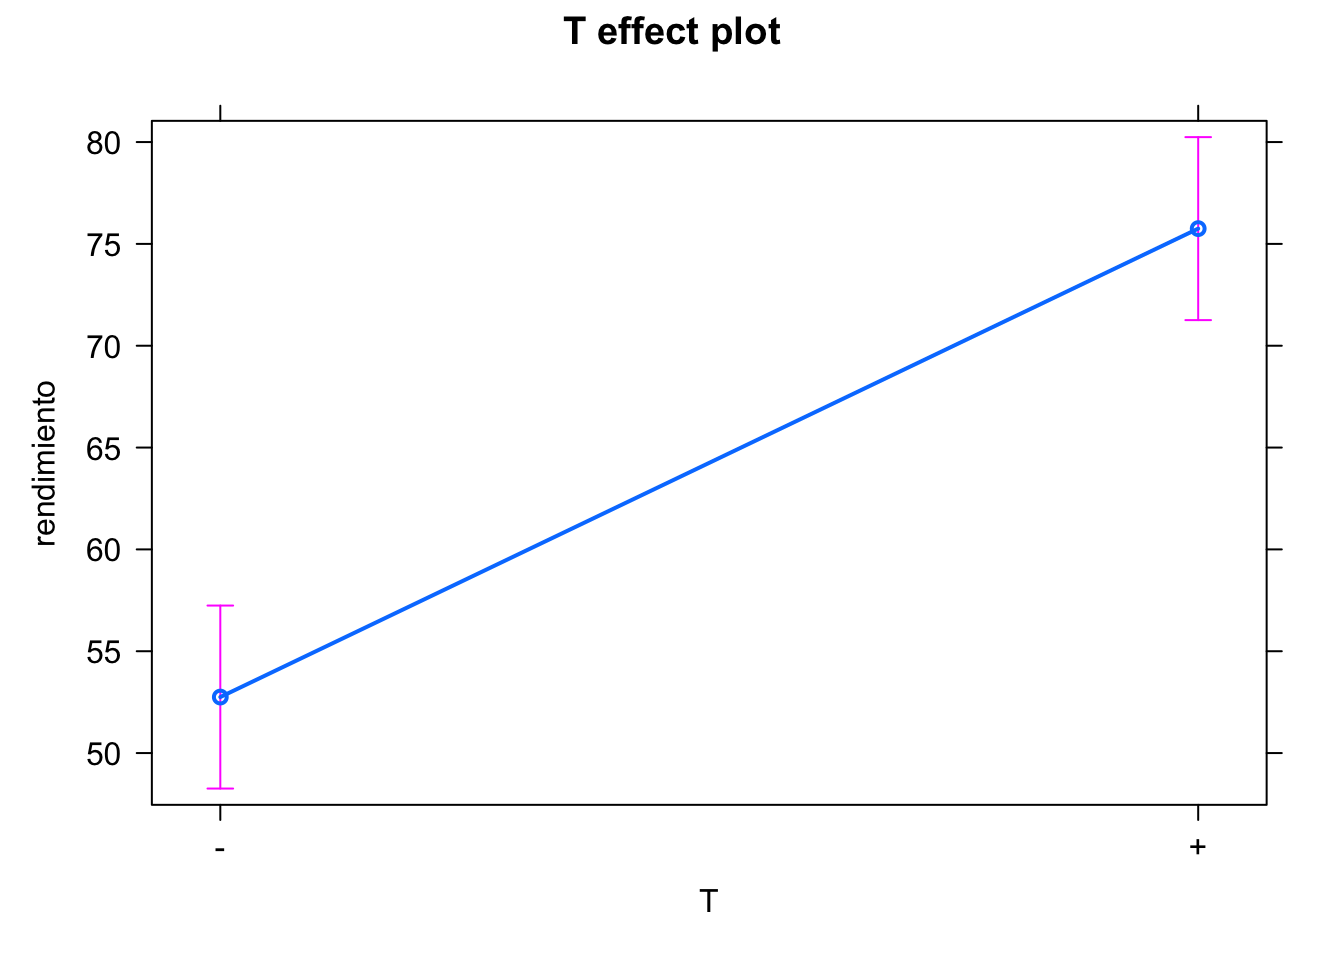
\includegraphics{91-apendices_files/figure-latex/unnamed-chunk-12-1.pdf}

\hypertarget{modelos-de-distribuciuxf3n-de-probabilidad-multivariantes}{%
\section{Modelos de distribución de probabilidad multivariantes}\label{modelos-de-distribuciuxf3n-de-probabilidad-multivariantes}}

\hypertarget{modelos-de-distribuciuxf3n-de-probabilidad-relacionadas-con-la-normal}{%
\section{Modelos de distribución de probabilidad relacionadas con la normal}\label{modelos-de-distribuciuxf3n-de-probabilidad-relacionadas-con-la-normal}}

\hypertarget{simulaciuxf3n-de-variables-aleatorias}{%
\section{Simulación de variables aleatorias}\label{simulaciuxf3n-de-variables-aleatorias}}

\(U(0;\; 1)\): Generador de probabilidades aleatorias. Dada cualquier función de distribución \(F\), se pueden generar valores de esa VA obteniendo \(F^{-1}(U(0;\; 1))\)

\hypertarget{demostraciones}{%
\chapter{Demostraciones}\label{demostraciones}}

Em este apéndice se incluyen aquellas demostraciones de teoremas y propiedades
no incluidas en los capítulos para mantener el carácter práctico del mismo.

\hypertarget{variable-aleatoria-discreta}{%
\section{Variable aleatoria discreta}\label{variable-aleatoria-discreta}}

\hypertarget{funciuxf3n-de-probabilidad}{%
\subsection{Función de probabilidad}\label{funciuxf3n-de-probabilidad}}

\hypertarget{esperanza}{%
\subsection{Esperanza}\label{esperanza}}

\hypertarget{varianza}{%
\subsection{Varianza}\label{varianza}}

\hypertarget{creditos}{%
\chapter{Créditos}\label{creditos}}

Los gráficos y diagramas generados son creación y propiedad del autor, salvo que se
indique lo contrario. Su licencia de uso es la misma que la del resto de la
obra, véase el Prefacio.

La \href{https://pixabay.com/es/illustrations/fondo-abstracto-l\%C3\%ADnea-ilustración-2462436/}{imagen de la portada} es de dominio público, obtenida en \href{https://pixabay.com/es/}{pixabay.com}, gracias al
usuario \href{https://pixabay.com/es/users/manuchi-1728328/}{Manuchi}.

Las imágenes de tipo \emph{clipart} usadas en esta obra y las fotografías no atribuidas
pertenecen al dominio público gracias a \href{http://www.openclipart.org}{openclipart.org}, \href{https://unsplash.com}{unplash.com} o \href{https://pixabay.com/es/}{pixabay.com}.

The \href{https://www.r-project.org/logo/}{R logo} is (c) 2016 The R Foundation.

  \bibliography{book.bib,packages.bib}

\end{document}
